\section{Joins}
\say{\(Non\)-Equi-joins, Auto-joins, Date\&Time Functies}

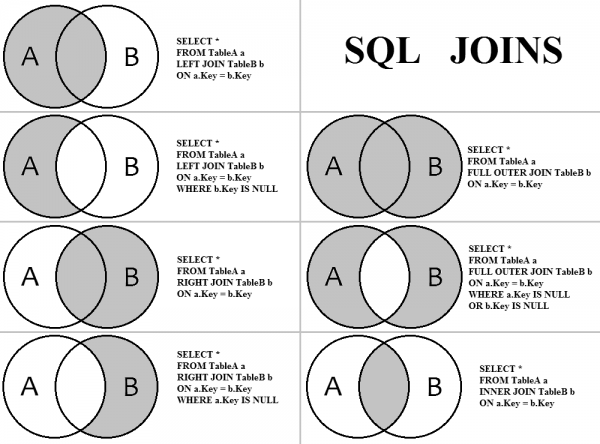
\includegraphics[scale=0.37]{./joins.png}

\subsection{Gewone JOIN}
Resulteert enkel gematchte records.
\begin{tiny}
\begin{lstlisting}
  SELECT * FROM foo f
  [INNER] JOIN bar b -- INNER is default
  ON f.id = b.id
\end{lstlisting}

\begin{lstlisting}
  SELECT * FROM foo
  JOIN bar USING(id) -- kolomnamen hebben dezelfde naam
\end{lstlisting}

\subsection{Non-equi JOIN}
\begin{lstlisting}
  SELECT first_name, last_name, schaalnr
  FROM employees
  JOIN pay_grades ON (salary/12 BETWEEN lower_limit AND upper_limit);

  -- De join is niet gebaseerd op een gelijkheid tussen attribuutwaarden
\end{lstlisting}
\end{tiny}

\subsection{Outer JOIN}
Resulteert in alle gematchte records + null lijnen.

\subsection{Auto JOIN}
Een gewone join, waarbij de tafel met zichzelf samenvoegt.
\say{Oftewel een "recursieve relatie"}

\begin{tiny}
\begin{lstlisting}
  SELECT *
  FROM employees e
  JOIN employees mgr
  ON (e.manager_id=mgr.employee_id);
\end{lstlisting}
\end{tiny}

\subsection{Impliciete conversies}
\cm{cast(foo AS INT)}{Omzetten van tekst naar numeriek}
\cm{to\_char(123, '999')}{Omzetten van numeriek naar tekst}
\cm{to\_char(dob,'TMMonth')}{vertaalde datum naar tekst}

\subsection{Afronden van nummers}
\cm{round(15251.675)}{afgerond op het geheel}
\cm{round(15251.675,1)}{afgerond op 1 decimaal}
\cm{round(15251.675,-1)}{afgerond tot een tiental}

\subsection{Afkappen van nummers}
\cm{trunc(15251.675)}{afgekapt op 1 geheel}
\cm{trunc(15251.675,1)}{afgekapt op 1 decimaal}
\cm{trunc(15251.675,-1)}{afgekapt op 1 tiental}

\subsection{Datum functies}
\cm{current\_date}{huidige datum}
\cm{date\_part}{stuk uit datum halen}
\cm{date\_trunc}{datum afhakken}

\subsection{Leeftijd}
\begin{tiny}
\begin{lstlisting}
  SELECT age(dob) "age" FROM employees;
  SELECT date_part('year',(age(dob))) FROM employees;
\end{lstlisting}

\subsection{Rekenen met datum \& tijd}
\begin{lstlisting}
  SELECT date '2021-09-28' + 7;
  SELECT date '2021-09-28' + interval '10 hour';
  SELECT time '01:00' + interval '3 hours';
  SELECT interval '1 hour' / 1.5;
\end{lstlisting}
\end{tiny}